%%%%%%%%%%%%%%%%%%%%%%%%%%%%%%%%%%%%%%%%%%%%%%%%%%%%%%%%%%%%%%%%%%%%%%
% LaTeX Template: Project Titlepage
%
% Source: http://www.howtotex.com
% Date: April 2011
% 
% This is a title page template which be used for articles & reports.
% 
% Feel free to distribute this example, but please keep the referral
% to howtotex.com
% 
%%%%%%%%%%%%%%%%%%%%%%%%%%%%%%%%%%%%%%%%%%%%%%%%%%%%%%%%%%%%%%%%%%%%%%
% How to use writeLaTeX: 
%
% You edit the source code here on the left, and the preview on the
% right shows you the result within a few seconds.
%
% Bookmark this page and share the URL with your co-authors. They can
% edit at the same time!
%
% You can upload figures, bibliographies, custom classes and
% styles using the files menu.
%
% If you're new to LaTeX, the wikibook is a great place to start:
% http://en.wikibooks.org/wiki/LaTeX
%
%%%%%%%%%%%%%%%%%%%%%%%%%%%%%%%%%%%%%%%%%%%%%%%%%%%%%%%%%%%%%%%%%%%%%%
%
% --------------------------------------------------------------------
% Preamble
% --------------------------------------------------------------------
\documentclass[paper=a4, fontsize=11pt,twoside]{scrartcl}	% KOMA

\usepackage[a4paper,pdftex]{geometry}	% A4paper margins
\usepackage{setspace}  
\setlength{\oddsidemargin}{5mm}			% Remove 'twosided' indentation
\setlength{\evensidemargin}{5mm}

\usepackage[english]{babel}
\usepackage[protrusion=true,expansion=true]{microtype}	
\usepackage{amsmath,amsfonts,amsthm,amssymb}
\usepackage{graphicx}
\usepackage{mathtools}
\usepackage{hyperref}
% --------------------------------------------------------------------
% Definitions (do not change this)
% --------------------------------------------------------------------
\newcommand{\HRule}[1]{\rule{\linewidth}{#1}} 	% Horizontal rule

\makeatletter							% Title
\def\printtitle{%						
    {\centering \@title\par}}
\makeatother									

\makeatletter							% Author
\def\printauthor{%					
    {\centering \large \@author}}				
\makeatother							

% --------------------------------------------------------------------
% Metadata (Change this)
% --------------------------------------------------------------------
\title{	\normalsize \textsc{MIP Project} 	% Subtitle
		 	\\[2.0cm]								% 2cm spacing
			\HRule{0.5pt} \\						% Upper rule
			\LARGE \textbf{\uppercase{Statistical Shape Analysis of Anatomical Structures}}	% Title
			\HRule{2pt} \\ [0.5cm]		% Lower rule + 0.5cm spacing
			\normalsize \today			% Todays date
		}

\author{Sushant 110050009\\
        Nilesh 110050007\\
        Sanchit 110050035\\
		Department of Computer Science and Engineering\\
        IIT Bombay\\
}


\begin{document}
% ------------------------------------------------------------------------------
% Maketitle
% ------------------------------------------------------------------------------
\thispagestyle{empty}		% Remove page numbering on this page

\printtitle					% Print the title data as defined above
  	\vfill
\printauthor				% Print the author data as defined above
\newpage
% ------------------------------------------------------------------------------
% Begin document
% ------------------------------------------------------------------------------
\tableofcontents
\newpage
\setcounter{page}{1}		% Set page numbering to begin on this page
\section{Introduction}
An important goal in image analysis is to classify and recognize objects of interest in given images. Imaged objects can be characterized in several ways, using their colors, textures, shapes, movements, and locations.
\\

Statistical shape analysis is a geometrical analysis from a set of shapes in which statistics are measured to describe geometrical properties from similar shapes or different groups, for instance, the difference between male and female Gorilla skull shapes, normal and pathological bone shapes, etc. Some of the important aspects of shape analysis are to obtain a measure of distance between shapes, to estimate average shapes from a (possibly random) sample, also called mean shape, and to estimate shape variability in a sample.

\subsection{Problem Statement}
This project focuses on estimating the mean shape, given various shapes. The given shapes can be rotated, scaled, translated versions of each other with some error (introduced possibly during annotations).
\\
To test our code, we used 2 types of data: 
\begin{itemize}
\item Automatically generated data comprising of ellipses with differing major-axis, minor-axis and rotation w.r.t the X-Y axos
\item A dataset comprising of annotated 
images. It consists of 56 points per image and 40 such images.
\item A dataset comprising of annotated Right Ventricle of Heart. This images were annotated by us as opposed to that of previous case wherein the data was annotated before hand. We used 12 points per image and annotated 10 such images.
\end{itemize}

\newpage
\section{Algorithm Used}
To completely understand the algorithms used, we will first define some terms.
\begin{itemize}
\item \textbf{Shape} is all the geometrical information that remains when location,
scale and rotational effects are filtered out from an object.
\item The \textbf{Shape Space} is the set of all possible shapes of the object in question
\item \textbf{The Procrustes distance} is a least-squares type shape metric that requires two aligned shapes with
one-to-one point correspondence
\end{itemize}

\subsection{Procrustes Analysis}
The alignment of images involves four steps:
\begin{itemize}
\item Compute the centroid of each shape.
\item Re-scale each shape to have equal size.
\item Align w.r.t. position the two shapes at their centroids.
\item Align w.r.t. orientation by rotation
\end{itemize}

The Procrustes Distance between 2 images $x_{1}$ and $x_{2}$ is given by:

$$ P_{d}^2 = \sum\limits_{j=1}^n [(x_{j1} - x_{j2})^2 + (y_{j1} - y_{j2})^2] $$ 

The centroid of the shape is found out as follows:

$$ (X,Y) = (\frac{1}{n} \sum\limits_{j=1}^n x_{j} , \frac{1}{n} \sum\limits_{j=1}^n y_{j})$$

To align 2 shapes together, Single Value Decomposition is applied.
\begin{itemize}
\item Arrange the size and position aligned $x_{1}$ and $x_{2}$ as $nx2$ matrices.
\item Calculate the SVD, UDVT, of $x_{1}^Tx_{2}$ in order to maximize the correlation between the two sets of landmarks.
\item The rotation matrix needed to optimally superimpose $x_{1}$ upon $x_{2}$ is then $VU^T$. i.e $VU^T$ is the rotation matrix.
\end{itemize}

\subsection{Generalized Procrustes Analysis}
This is essentially an interative approach using the Procrustes Method.
It is done as follows:
\begin{itemize}
\item Choose an initial estimate of the mean shape (we chose the first shape in the set).
\item Align all the remaining shapes to the mean shape.
\item Re-calculate the estimate of the mean from the aligned shapes.
\item If the estimated mean has changed return to step 2.
\end{itemize}


\section{Experiments}
The following subsections will show in detail the result of using the algorithm.

\subsection{Hand Data}
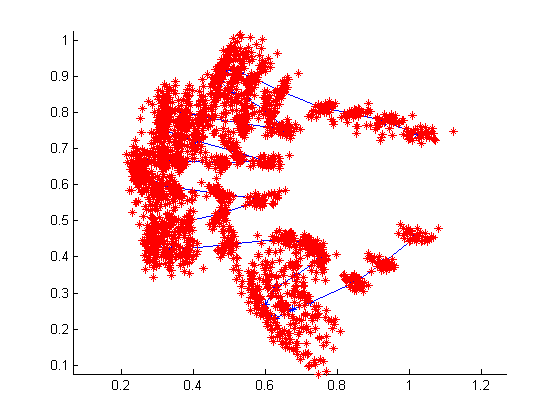
\includegraphics{HandMeanwithData.png}
This image shows the Scaled Data Points for all the annotated hand images in red and the final mean data in blue. The mean shape has been joined together just for further clarity.

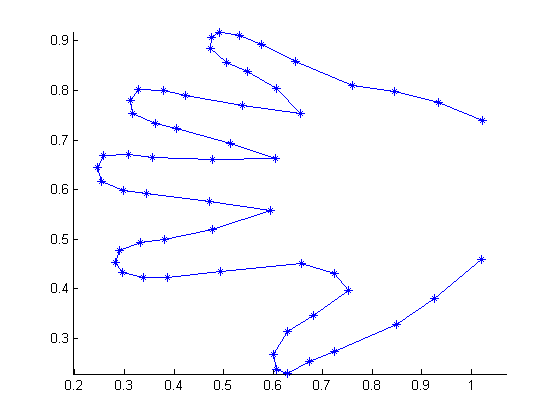
\includegraphics{HandMean.png}
The mean hand shape which was buried beneath the scaled data points in previous image.

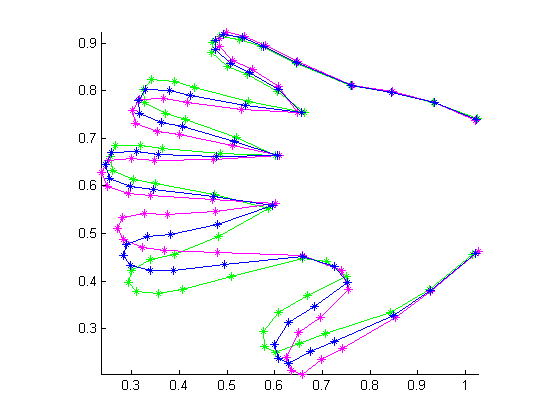
\includegraphics{HandMode1.png}
Blue colored is the mean hand. The green color is $Mean - \sqrt{\lambda}$ and the Magenta is $Mean + \sqrt{\lambda}$ This is the mode1 image formed corresponding to the largest eigen value. 

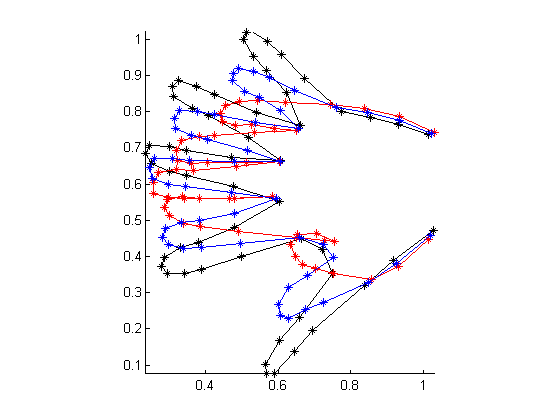
\includegraphics{HandMode2.png}
Blue colored is the mean hand. The red color is $Mean - \sqrt{\lambda}$ and the black is $Mean + \sqrt{\lambda}$. This image is corresponding to the second highest eigen value. As we can see, the red color variant tries to describe fingers held together whereas the black variant describes fingers stretching outwards.

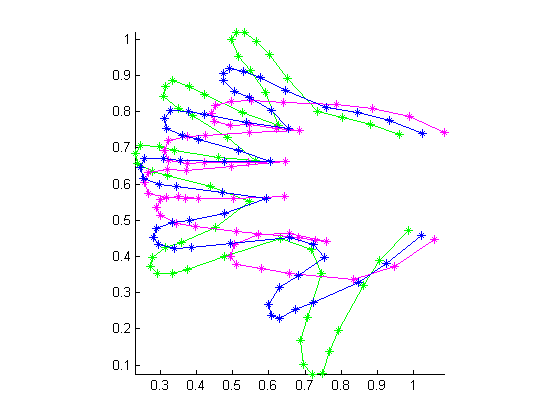
\includegraphics{HandMode3.png}
Blue colored is the mean hand. The green color is $Mean - \sqrt{\lambda}$ and the Magenta is $Mean + \sqrt{\lambda}$. This image is corresponding to the $3^{rd}$ highest eigen value. In continuance with the previous description, the green colored variant is a bit more wider and the magenta variant is a bit more close knit.

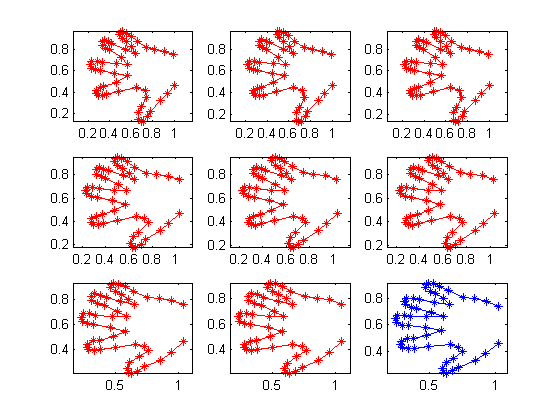
\includegraphics{HandSubplot.png}
The $1^{st}$ 7 images show annotated Hand images, the last image shows the Calculated Mean Hand Shape. The scales of all the images are same and hence we can compare the given data with the final Mean Shape.

\subsection{Heart Data}
We manually annotated right ventricle of heart using 12 points. We annotated 10 such images.
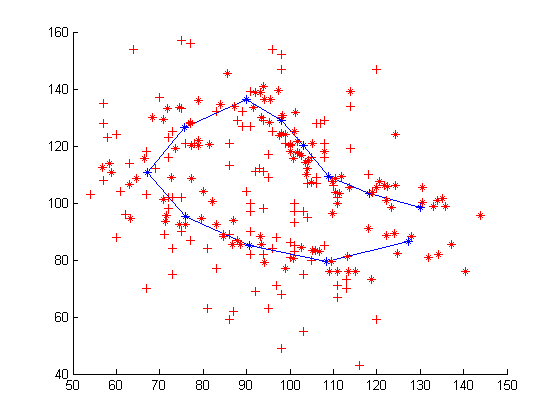
\includegraphics{HeartMeanwithData.png}
The red points show the annotated right ventricle data whereas the blue data shows the mean image. This data appears more scattered as opposed to that of Hand Data, this is primarily because it was annotated manually by us.

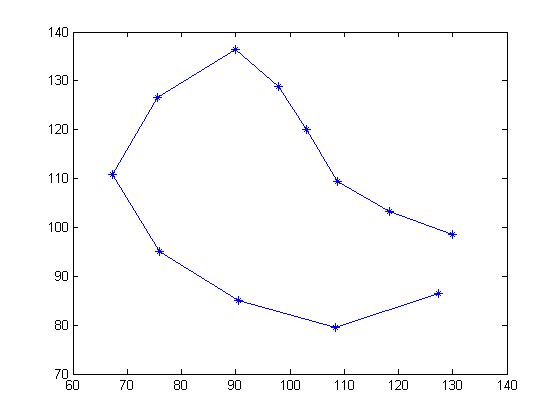
\includegraphics{HeartMean.png}
Carrying forward the previous image, the blue points show the Mean Right Ventricle Shape.

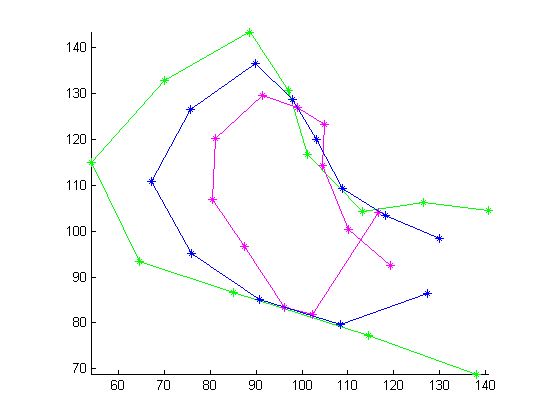
\includegraphics{HeartMode1.png}
Blue colored is the mean Right Ventricle. The green color is $Mean - \sqrt{\lambda}$ and the Magenta is $Mean - \sqrt{\lambda}$. This is the mode1 image formed corresponding to the largest eigen value. 

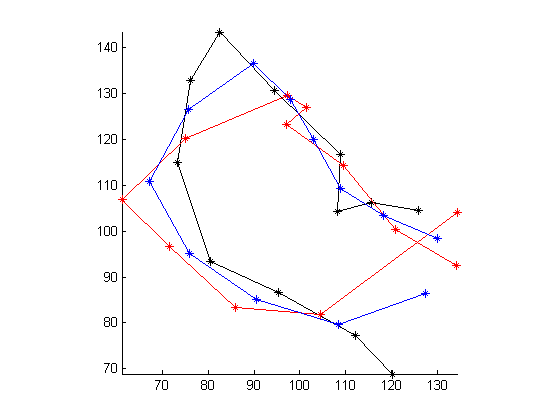
\includegraphics{HeartMode2.png}
Blue colored is the mean right ventricle shape. The red color is $Mean - \sqrt{\lambda}$ and the black is $Mean + \sqrt{\lambda}$. This image is corresponding to the second highest eigen value.

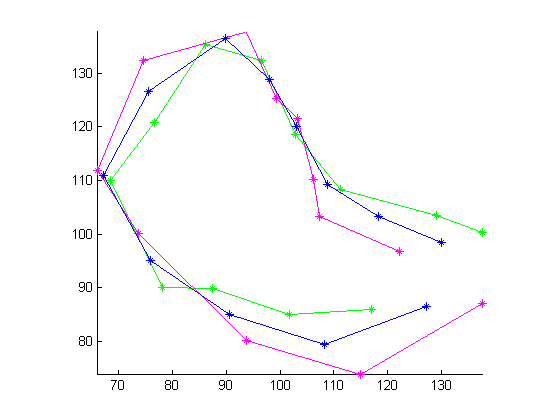
\includegraphics{HeartMode3.png}
Blue colored is the mean Right Ventricle. The green color is $Mean - \sqrt{\lambda}$ and the Magenta is $Mean - \sqrt{\lambda}$ This image is corresponding to the third highest eigen value.


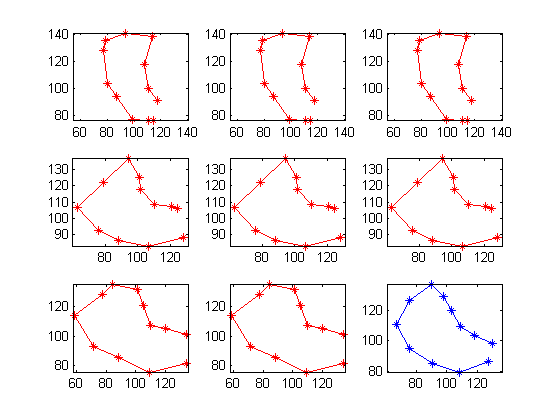
\includegraphics{HeartSubplot.png}
Right Ventricle annotated data in comparison with the Calculated Mean Shape. All the images have same scale.

\section{Observations and Conclusions}
\subsection{Observations}
As can be seen from the previousgeneralized Procrustes analysis works very well in generating the mean Shape from a group of images. We as well verified the generated images from some of our friends (Visual inspection). They were all satisfied with the mean shapes generated using Procrustes Analysis. Also the images generated are comparable to the results obtained in the Standford Paper[1]

\subsection{Future Works}
\begin{itemize}
\item The algorithm used can be improved further if we use Tangent Space Projection. In this method instead of projecting the points on a hypersphere, they are projected on a plane perpendicular to the hypersphere. Although theorotically this should be true, practical implementations of this method are not as successful.
\item Also for improved version of statistical analysis, PCA can be used.
\end{itemize}

\subsection{Acknowledgement}
We would like to thank Prof. Suyash Awate for guiding us in choosing the project topic and always giving us advice regarding the progress of the project and solving our doubts.

\subsection{Bibliography}
[1] A brief Introduction to Statistical Shape Analysis 
\url{http://graphics.stanford.edu/courses/cs164-09-spring/Handouts/paper_shape_spaces_imm403.pdf}
\newline
[2] Annotated Data Sets of Hand and Heart. 
\url{http://www2.imm.dtu.dk/~aam/}
\end{document}